%! Author = mariuszindel
%! Date = 25.01.21

\section{Signalparameter}


\subsection{Was ist Information?}
\begin{center}
    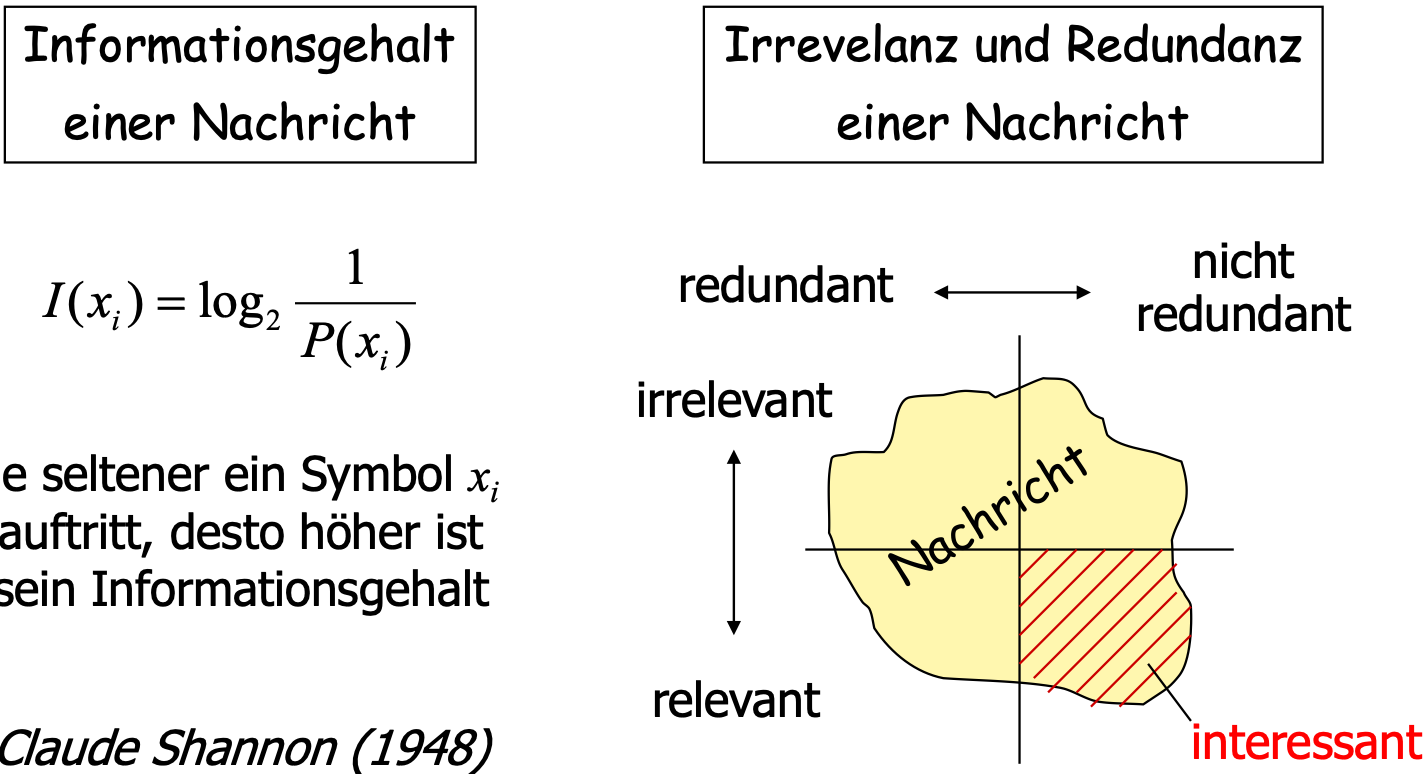
\includegraphics[width=\linewidth]{graphic/signalparameter/wasist.png}
\end{center}
\vspace{-8pt}


\subsection{Non-Return-to-Zero Code (NRZ)}
\subsubsection{gleichstrombehaftet, keine Taktinformation}
\begin{center}
    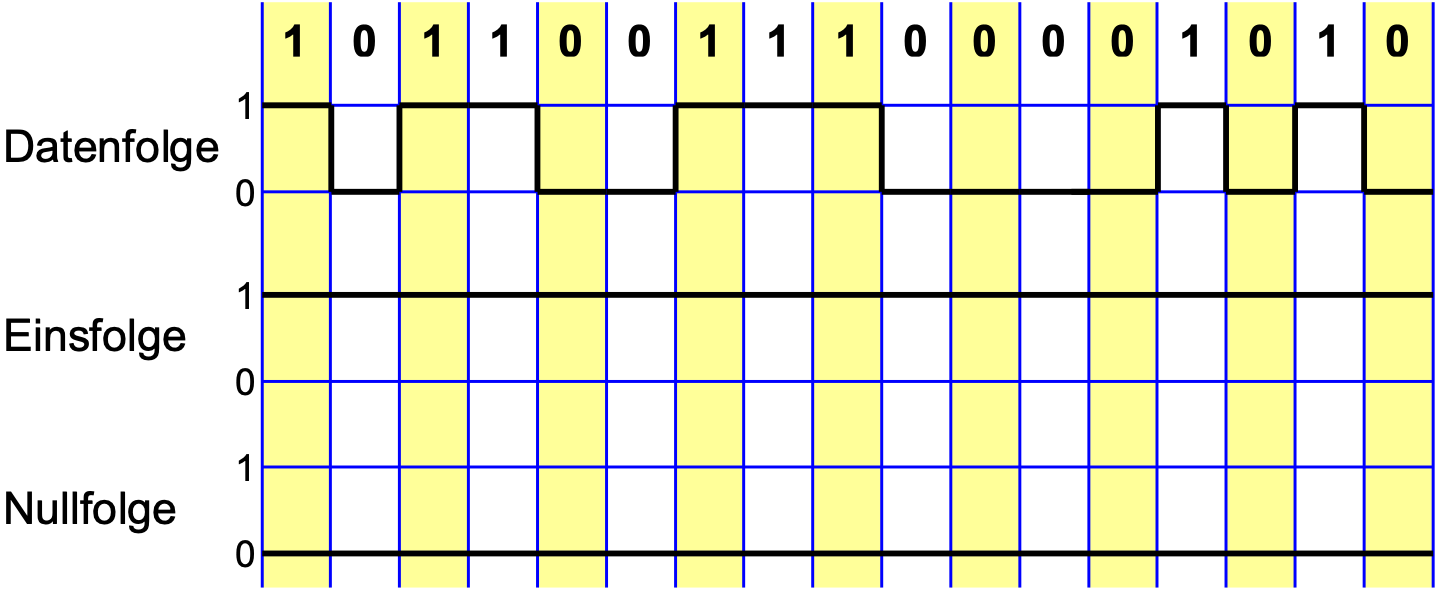
\includegraphics[width=\linewidth]{graphic/signalparameter/gleichstrombehaftet.png}
\end{center}
\vspace{-8pt}

\subsubsection{gleichstromfrei, volle Taktinformation}
\begin{center}
    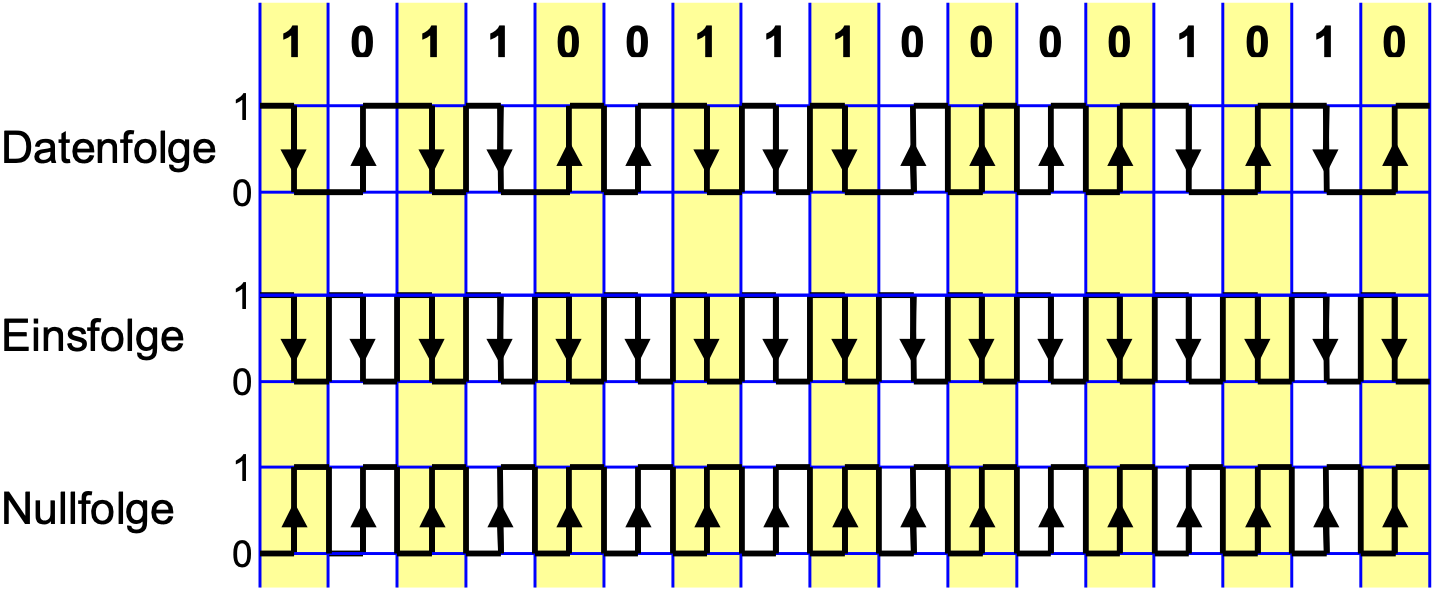
\includegraphics[width=\linewidth]{graphic/signalparameter/gleichstromfrei.png}
\end{center}
\vspace{-8pt}

\subsection{Pegelberechnung}
 \begin{center}
     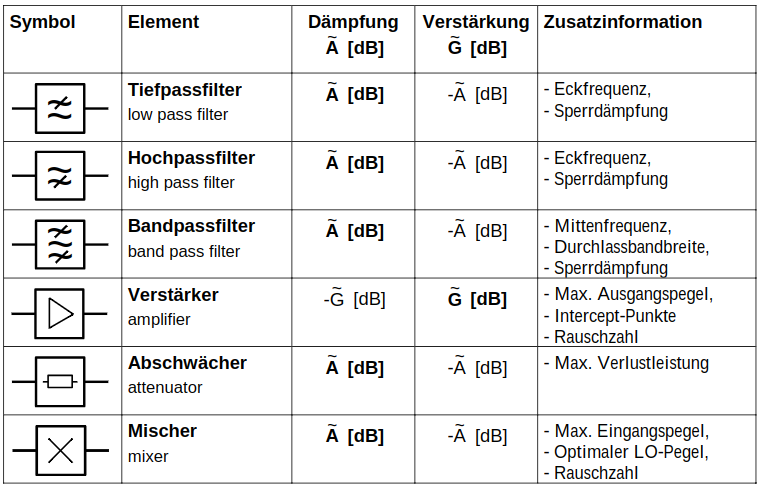
\includegraphics[width=\linewidth]{graphic/signalparameter/pegelplan.png}
 \end{center}
 \vspace{-8pt}

\subsubsection{Maximaler Ausgangspegel (z.B für Vorverstärker)}
$P=\frac{\hat{U}^{2}}{2 R}=\frac{(1 \mathrm{~V})^{2}}{2 \cdot 50 \Omega}=10 \mathrm{~mW} $\\
$\quad \widetilde{P}[\mathrm{dBm}]=10 \cdot \log \frac{P}{1 \mathrm{~mW}}=\underline{\underline{10 \mathrm{dBm}}}$


\subsubsection{Signaldynamik}
Differenz zwischen höchst- und tiefstmöglichen Pegel
\vspace{-8pt}
\begin{center}
    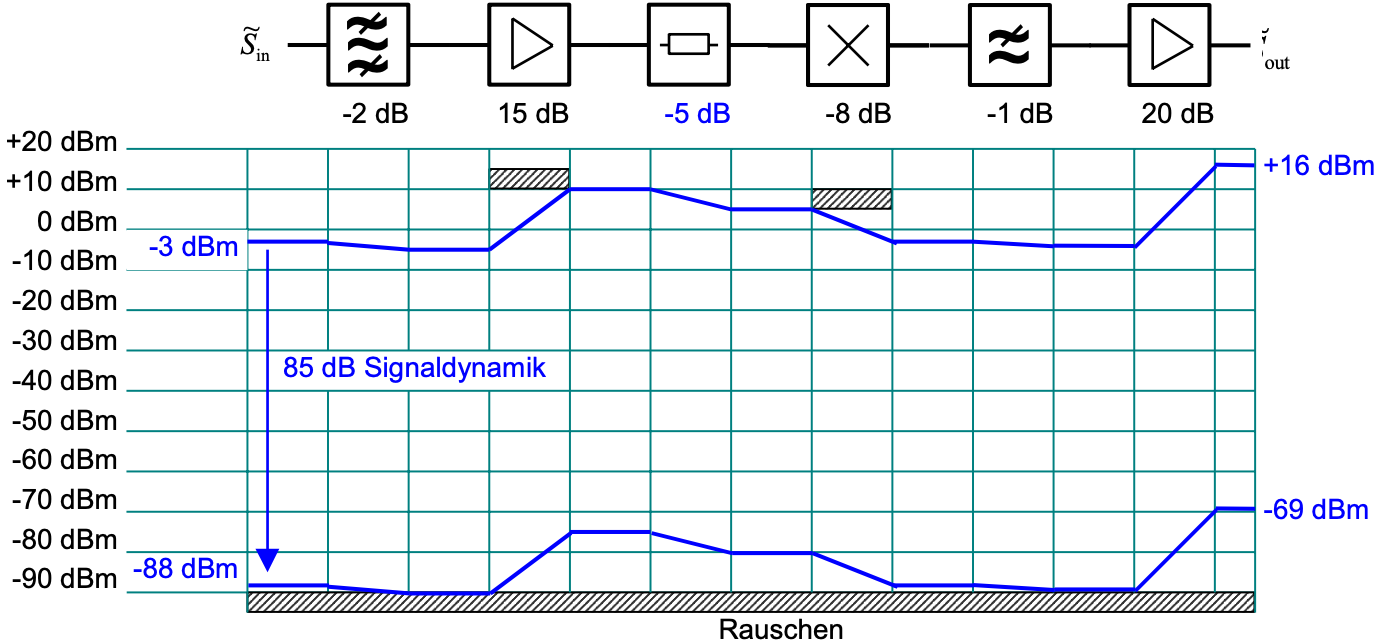
\includegraphics[width=\linewidth]{graphic/signalparameter/uebung.png}
\end{center}
\vspace{-8pt}


\subsubsection{Spannungseffektivwert}
$\widetilde{P}_{\max }=+16 \mathrm{dBm} \rightarrow \quad P_{\max }=40 \mathrm{~mW} $\\
$\quad U_{\max }=\sqrt{R P_{\max }}=\sqrt{50 \Omega \cdot 0.04 \mathrm{~W}}=1.41 \mathrm{~V}_{\mathrm{eff}}$


\subsection{Watt $\rightarrow$ dBm}
$L_{P}[\mathrm{dBm}]=10 \log _{10}\left(\frac{P}{1 \mathrm{~mW}}\right)$
\vspace{-8pt}
\begin{center}
    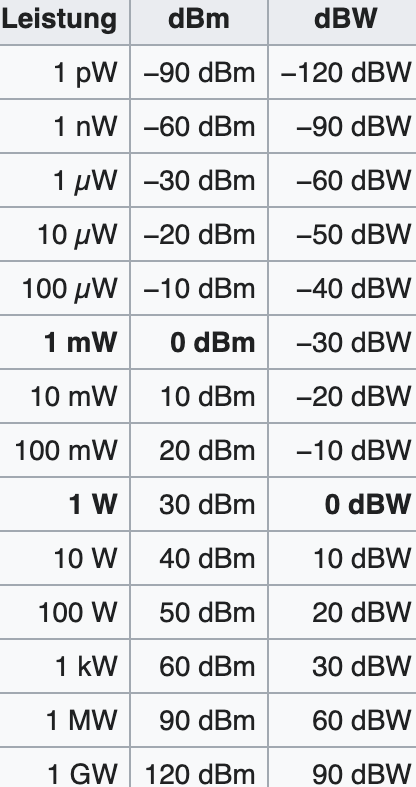
\includegraphics[scale=.3]{graphic/signalparameter/dbm-tabelle.png}
\end{center}
\vspace{-8pt}


\subsection{dBm $\rightarrow$ Watt}
$P[\mathrm{~mW}]=10^{\left(\frac{L_{P}[\mathrm{dBm}]}{10}\right)} \cdot 1 \mathrm{~mW}$
